%!TEX root = ../thesis.tex

\chapter{Grundlagen}
\label{chap:fundamentals}
\todo{Grundlagen einteilen und schreiben}
In diesem Kapitel werden die Grundlagen erläutert, die für das Verständnis dieser Arbeit wichtig sind. 

Zum einen werden in \prettyref{sec:darts} die Grundlagen des Dartsportes erläutert, auf deren Wesen die Idee dieser Abhandlung fußt. Dabei wird vom Dartboard bis zu den Darts und den allgemeinen Turnierregeln ein Überblick gegeben, um den Nutzen und die Motivation verständlicher zu machen.

Weiterhin werden grundlegende Informationen der Bildverarbeitung vermittelt im \prettyref{sec:basics}. Es wird ebenfalls ein Überblick über die verwendeten Bibliotheken zur Implementierung gegeben.

Anschließend wird im \prettyref{sec:setup} das genutzte Testsetup dargestellt, welche für die praktische Implementierung genutzt wird.
\section{Dartsport}
\label{sec:darts}
Darts ist ein Spiel, das eine gute Geschicklichkeit und ein gutes Maß an Auge-Hand-Koordination erfordert. Dabei werden Pfeile,genannt Dart, mit der Hand auf eine Zielscheibe geworfen und Punkte erzielt. Damit es eine Regulierung über das Spielmaterial gibt hat der Dartsport im Jahr 1920 eine erste Standardisierung erhalten. Die 1924 gegründete "`National Dart Association"' hat diesen zum Standard ihrer Liga erklärt \autocite[5]{guide2013}. Diese Standardisierung findet sich in vielen heutigen Regelwerken der verschiedenen Verbänden wieder. Auch in der Sport- und Wettkampfordnung des Deutschen
Dart-Verband (DDV) \autocite{DartsRegel2016}. Aus dieser sind die Folgenden Erklärungen und Reglungen entnommen. 

Zunächst einmal zum Dartboard, das heutzutage genutzte Dartboard ist in Abbildung\prettyref{Fig:dartboard} zu sehen. In seiner heutigen Form wurde es zum Zeitpunkt der Standardisierung 1924 geschaffen. Die Größe des gesamten Boardes und der einzelnen Felder ist hierbei normiert und Standard. Wie in Abbildung \prettyref{Fig:dartboard} abzulesen. 

Heutzutage werden sogenannte Boards vom Typ "`Bristle"' verwendet. Dieser Name stammt vom englischen Wort für Bürste ab. Diese Board werden aus Sisal-Fasern gefertigt, welche in Aufprallrichtung der Pfeile aufgestellt sind, sodass die Pfeile sich zwischen die Fasern schieben können. \autocite[6]{dph2015}. Die Drähte, die die einzelnen Felder voneinander trennen werden "`Spider"' genannt.
\begin{figure}
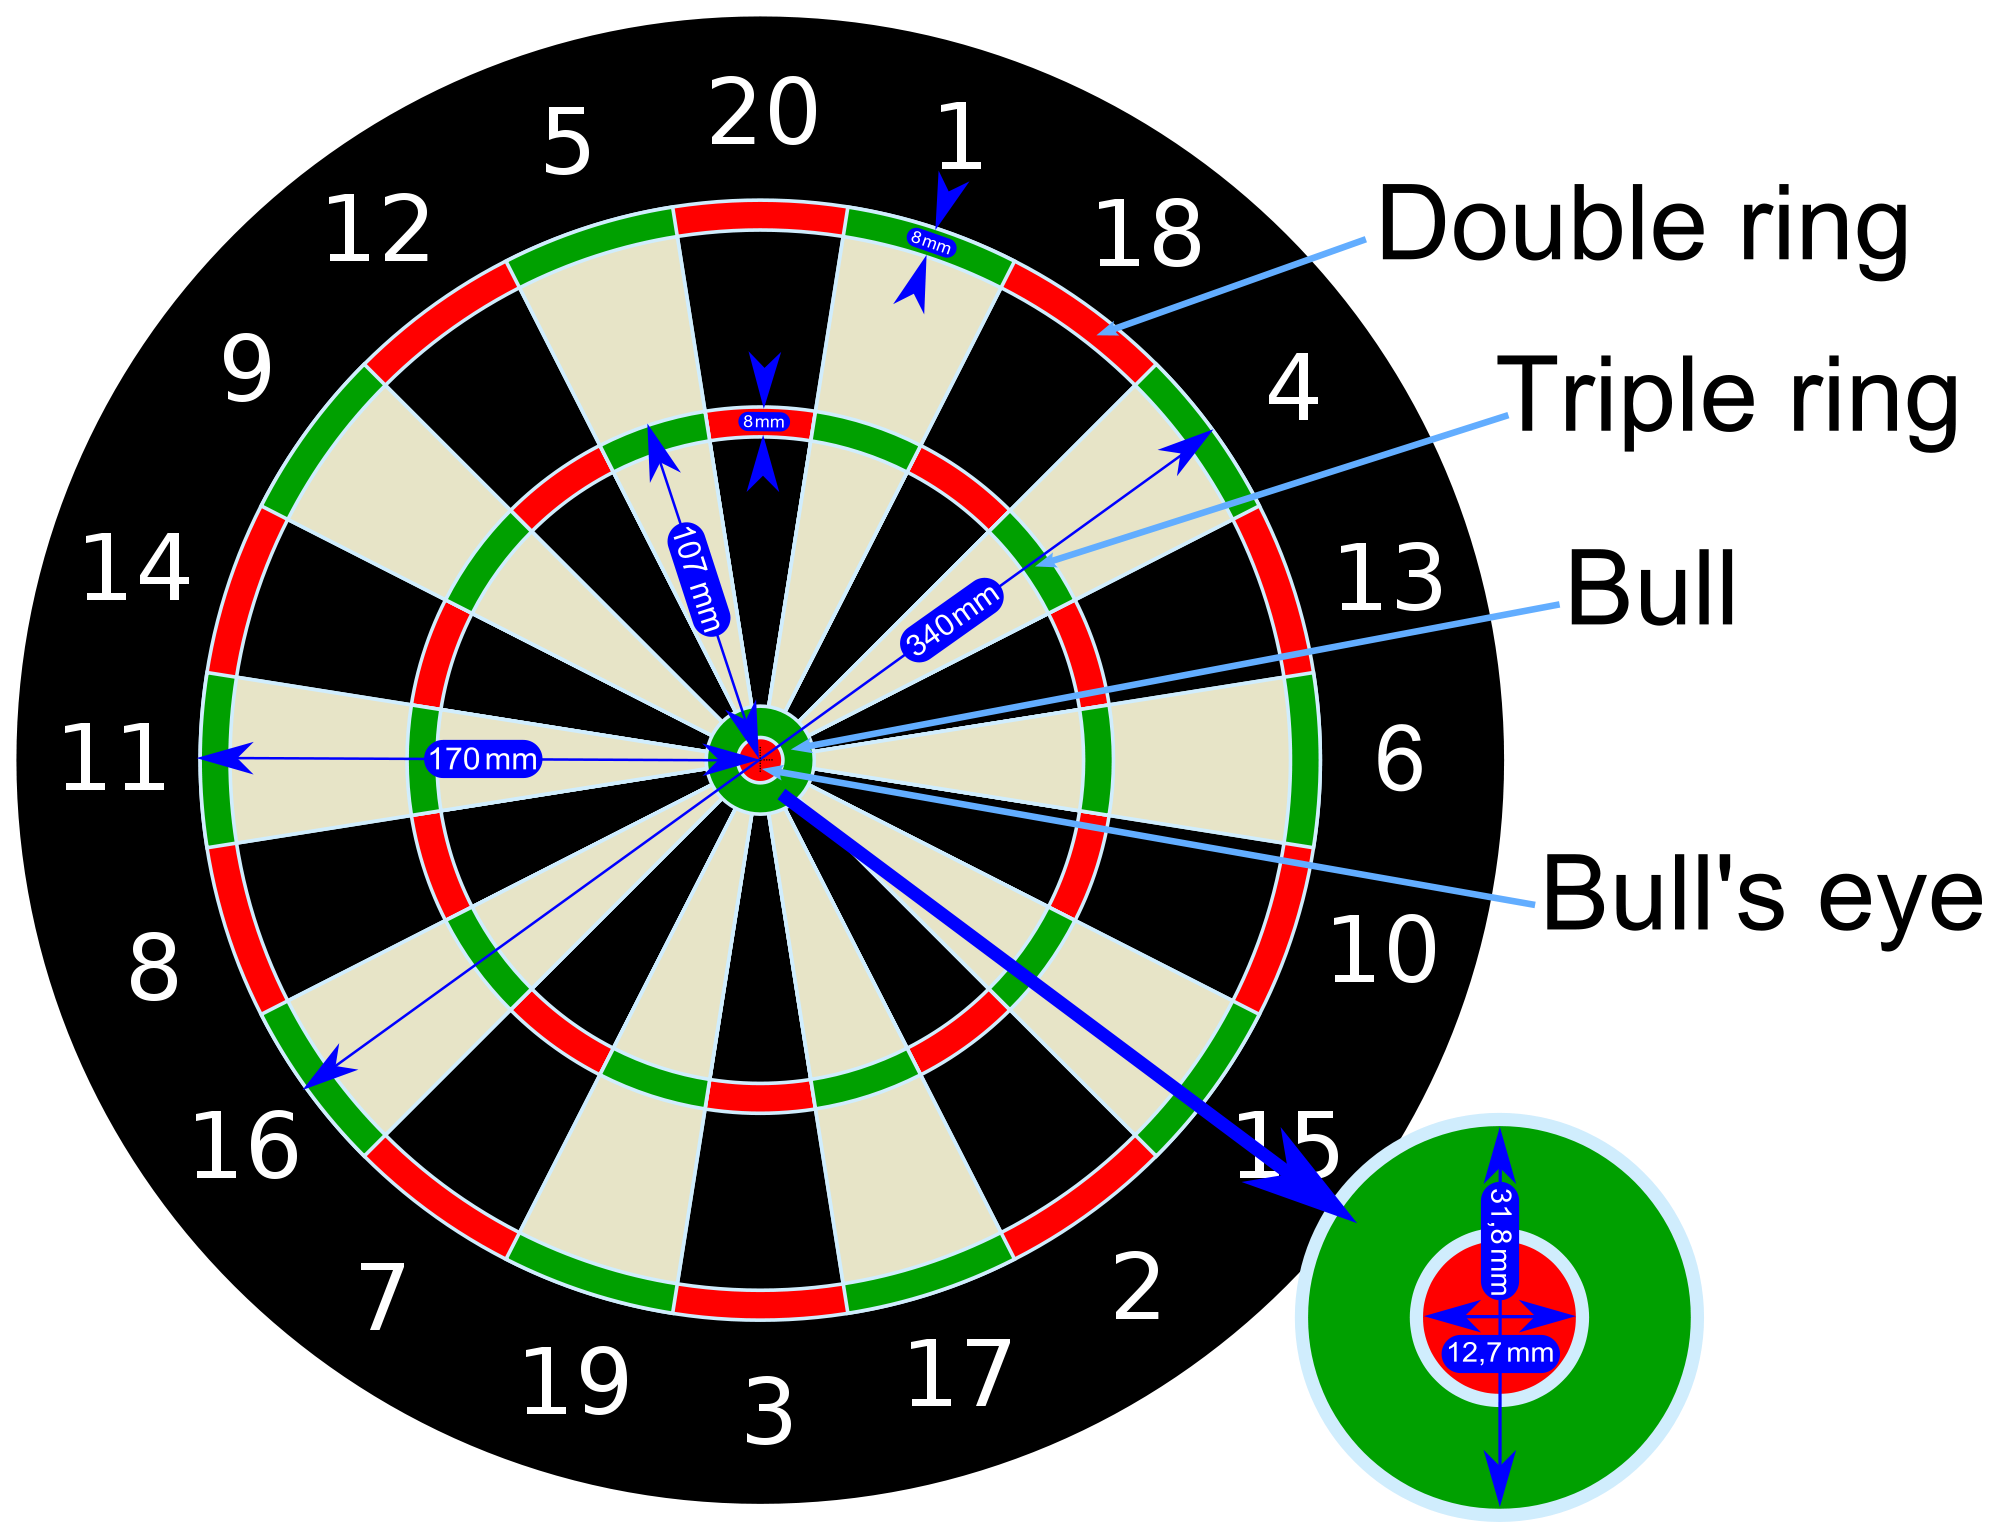
\includegraphics[width=\textwidth]{media/Dartboard_Abmessungen}\\
\caption{\textbf{Standardisiertes Dartboard\cite{Board2016}}
}
\label{Fig:dartboard}
\end{figure}

Die Anordnung der Ziffern ist hierbei von Oben im Uhrzeigersinn gelesen in der Folge 20-1-18-4-13-6-10-15-2-17-3-19-7-16-8-11-14-9-12-5. Diese wird als "`London Board"' bezeichnet. Hierbei wird der äußere 8mm breite Ring als "`Double Ring"' bezeichnet und und der innere als "`Triple Ring"' und verdreifacht die Punktzahl des Feldes. Der "`Bull"', der innere Bereich des Boards ist unterteilt in den grünen Teil genannt "`Half Bull"' and das "`Bullseye"', dieses zählen 25, bzw. 50 Punkte. 
Somit ist das "`Bullseye"' nicht, wie viele glauben, das Feld mit den meisten Punkten. Es gibt sogar gleich 4 Felder, die eine höhere Punktzahl erbringen, die Triple 20, 19, 18 und 17. Die Tripple 20 hat somit mit 60 Punkten die höchste zu erreichende Punktzahl. Im folgenden werden Triple Felder als "`TX"' bezeichnet, wobei X für die Ziffer des jeweiligen Feldes steht, zum Beispiel also T20. Eine weitere nennenswerte Schreibweise ist analog die für Doppelte Felder mit "`DX"'. 

\begin{figure}
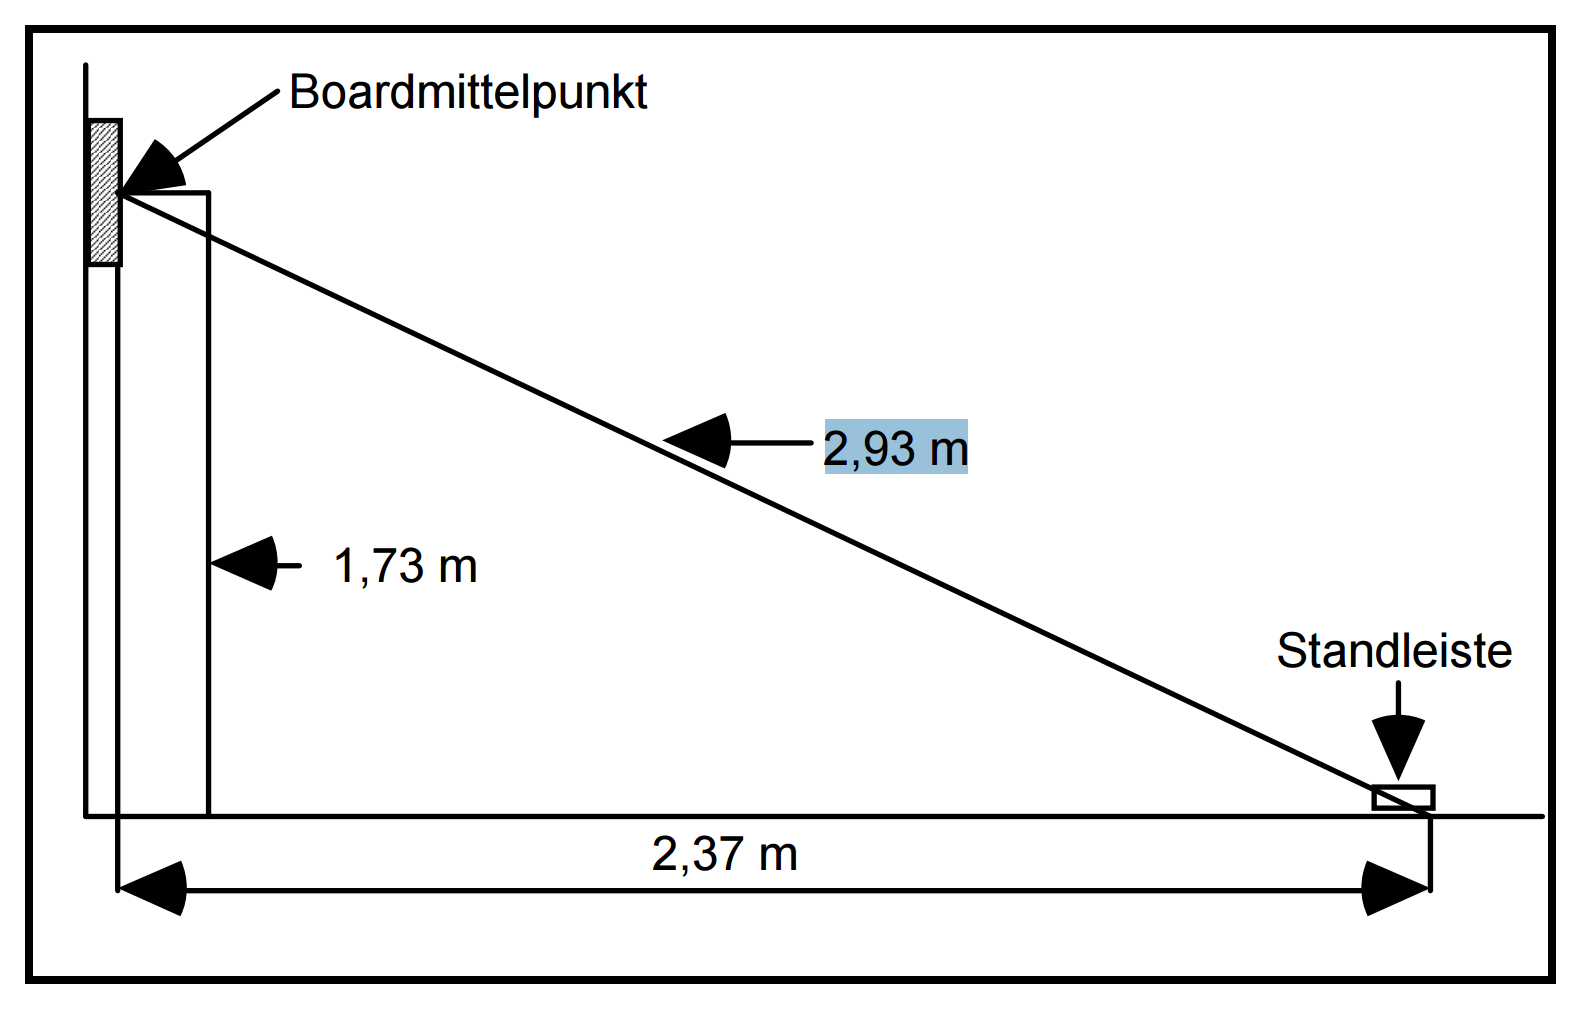
\includegraphics[width=\textwidth]{media/Dartsfield}\\
\caption{\textbf{Seitenansicht von Board und Standleiste 
\cite[8]{DartsRegel2016}}
}
\label{Fig:dartsetup}
\end{figure}


Das Board wird mit dem Mittelpunkt des "`Bullseyes"' auf eine Höhe von 1,73 gehängt, in der Weise, dass sich das Feld mit der 20 mittig oben befindet \autocite[6-8]{DartsRegel2016}. In Abbildung \prettyref{Fig:dartsetup} ist eine Seitenansicht einer Dartanlage nach dem Regelwerk des DDV zu sehen. Die Standleiste, oder "`Oche"' befindet sich hier in einer Entfernung von 2.37 zur Front-Seite des Boards. 

Als letzten Teil der Ausrüstung gilt es den Dart selbst zu beschreiben. Bei einem Dart, wie in Abbildung \prettyref{Fig:darts} zu sehen, sind grundsätzlich vier Hauptbestandteile zu unterscheiden:
\begin{enumerate}
    \item Point, Tip oder Spitze
    \item Barrel
    \addtocounter{enumi}{1}
    \item Shaft
    \addtocounter{enumi}{1}
    \item Flight
\end{enumerate}
\begin{figure}
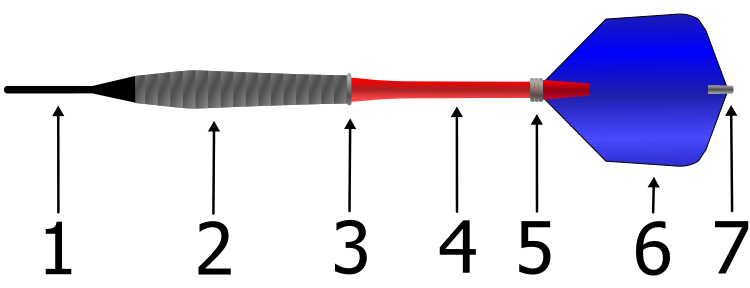
\includegraphics[width=\textwidth]{media/Dart}\\
\caption{\textbf{Aufbau eines Darts\cite{dart2006}}
}
\label{Fig:darts}
\end{figure}
Die weiteren Bestandteile sind optional und nicht zwingend notwendig für den Dart. 
\begin{enumerate}
	\addtocounter{enumi}{1}
	\addtocounter{enumi}{1}
    \item O-Ring, um den Shaft (4) fester im Barrel (2) zu befestigen
    \item Collar, dient dazu das Ende des Shafts zusammenzudrücken, um den Flight sicherer zu befestigen
    \addtocounter{enumi}{1}
    \item Flight Protector, dient dazu den Flight vor dem Auftreffen anderer Darts zu schützen

\end{enumerate}

Dart wird im Turniersport in zwei verschiedenen Modi gespielt, welche sich sehr ähneln. Zum einen gibt es 501 und zum anderen 301 im Modus "`Straight in"'  und  "`Double Out"'.

Beginnend beim sogenannten "`Leg"', hierbei hat zunächst jeder Spieler einen Pool von genannter Punktzahl. Dieser wird mit jedem erzielten Punkt verringert. Ziel ist es als erster Spieler die Punktzahl auf 0 zu reduzieren. Hierbei ist zu beachten, dass genau auf 0 heruntergespielt werden muss. Des weiteren gilt für das Beenden, das dies mit einem Doppel-Feld erzielt werden muss. Zusätzlich ist es auch möglich "`Bull Out"' zu erzielen, also nicht mit einem Doppelfeld abzuschließen, sondern mit dem "`Bullseye"'. Wird die Punktzahl mit einem Wurf, ein Wurf besteht aus den 3 Darts, auf 1 oder in den negativen Bereich gebracht so gilt es als überworfen und wird als "`Bust"' bezeichnet. In diesem Fall wird die Punktzahl vor dem Wurf wiederhergestellt. \autocite[5]{DartsRegel2016} 

Das Leg gewonnen hat der Spieler oder Team, der als erstes auf 0 herunter gespielt hat. Mehrere Legs werden zu einem "`Set"'  zusammengefasst. Der erste Spieler oder Team, der eine definierte Anzahl an Legs gewinnt, gewinnt ein Set. Sets fügen sich wiederum zu einem Match zusammen. Gewonnen ist ein Match von dem Spieler oder Team, das als erstes eine definierte Anzahl an Sets gewinnt.

\begin{example}[Ein Spieler hat 10 Punkte verbleibend] 

Es müsste eine D5 erzielt werden. Um mit dem ersten Dart abzuschließen. Im folgenden verschiedene Szenarien um die Regeln zu veranschaulichen.
\begin{enumerate}
	\item Es wird eine D5 geworfen, der Spieler gewinnt somit das Leg
	\item Es wird eine 8 erzielt. Der zu tilgende Punktestand beträgt somit 2 und es müsste eine D1 erzielt werden, um das Leg zu beenden. Der Spieler trifft im Anschluss die D1 und entscheidet das Leg somit für sich. 
	\item Es wird eine 8 erzielt. Der zu tilgende Punktestand beträgt somit 2. Statt der D1 wird eine einfach 1 erzielt und somit ist der Wurf ungültig und die Punktzahl wird auf 10 zurück gesetzt.
\end{enumerate}
\end{example}

Rechnerisch ist es bei 501 also möglich, mit 9 Darts zu beenden (3xT20, 3xT20, 2xT20+Bullseye) , der sogenannte "`Neun Darter"'.

Die bisher beschriebene Dart Variante ist wird als "`Steeldart"' bezeichnet, da die Darts in der Regel eine Stahlspitze besitzen und einen Metallshaft haben. Dem gegenüber gibt es noch das sogenannte "`Softdart"' \todo{Quelle einfügen}. Beim Softdart wird nicht mit Darts mit Stahlspitzen gespielt, sondern mit Kunststoffspitzen. Dem entsprechend ist auch das Board ein Kunststoffboard mit vorgefertigten Löchern, in die die Spitzen der Pfeile eindringen können. 

\section{Grundlagen Bildverarbeitung}
\label{sec:basics}
Im folgenden werden einige Grundlagen beschrieben, die nötig sind um die verwendeten Algorithmen und Vorgehen nachvollziehen zu können. Es wird davon ausgegangen das grundlegende Kenntnisse zum Aufbau eines digitalisierten Bildes vorhanden sind. 
\subsection{Physik und Geometrie einer Kamera}
\label{sec:camerageo}
Beginnend bei der Entstehung der Verarbeiteten Bilder. 

Zur Vereinfachung wird vorerst von dem sogenannten "`Pinhole Camera Model"' ausgegangen. In Abbildung \prettyref{Fig:simple-pinhole} ist ein solches Modell zu sehen. 

Mittig ist die Barriere zu sehen in derer sich ein Loch c befindet, durch das die Lichtstrahlen auf die Image Plane I treffen können. Daraus bildet sich ein auf dem Kopf stehendes Bild. $c$ ist hierbei das Zentrum des Koordinatensystem.
Die Distanz zwischen I und der Barriere $(f)$ ist bei heutigen Kameras die Focal Length. Hierbei gilt es zu bemerken, dass heute Kamera natürlich nicht mehr nur ein Loch besitzen, sondern eine Linse eingesetzt ist, die die Lichtstrahlen brechen und auf die Image Plane lenken. Das grundlegende Modell bleibt aber auch bei heutigen Kameras bestehen. Wie die Linse das Bild verändert wird später eingegangen. 

Auf diese Weise entsteht eine Abbildung des Punktes $P$ auf der zwei dimensionalen Fläche $I$. Sind alle Parameter bekannt lässt sich folglich bestimmten, wo der Punkt $P$ später im Bild zu sehen sein wird. 

\begin{figure}
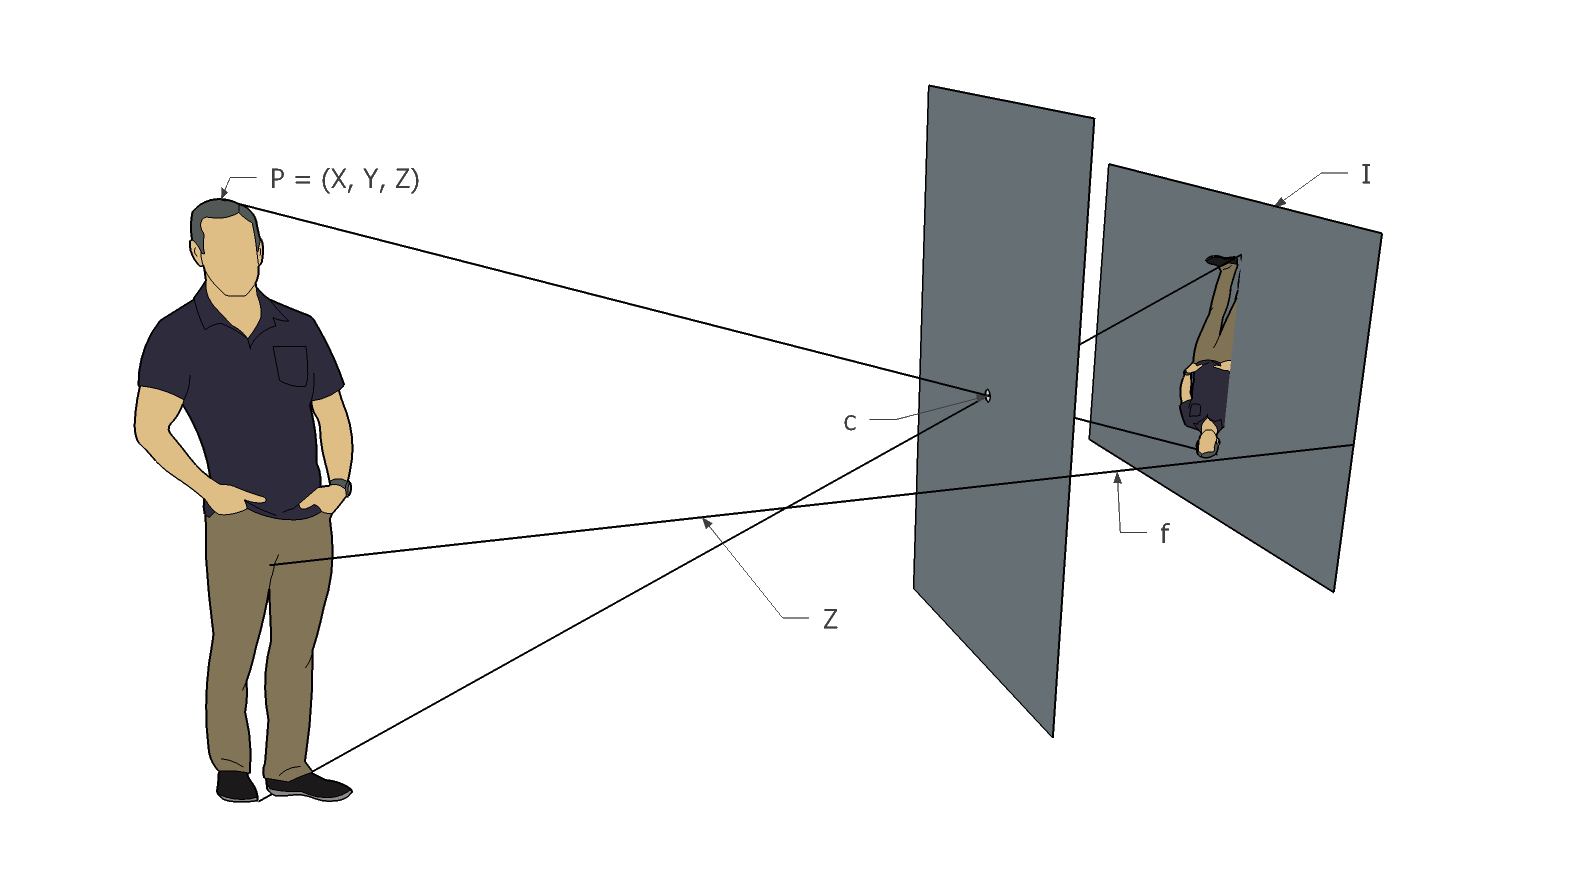
\includegraphics[width=\textwidth]{media/simple-pinhole.png}\\
\caption{\textbf{Einfache Darstellung, der Funktionsweise einer einfachen Loch Kamera}
}
\label{Fig:simple-pinhole}
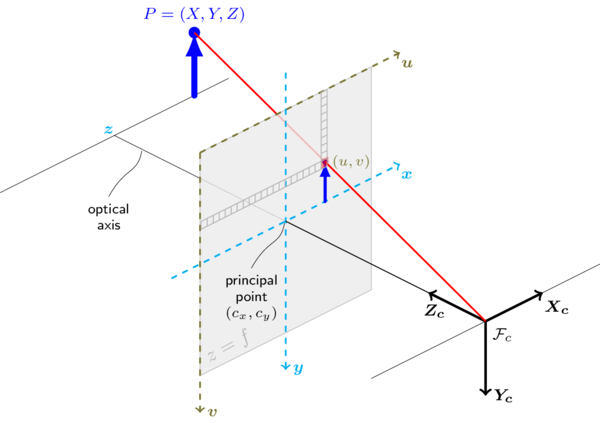
\includegraphics[width=\textwidth]{media/pinhole_camera_model}\\
\caption{\textbf{Pinhole Camera Modell von.\autocite{OpencvCamera2016}}
}
\label{Fig:pinhole}
\end{figure}

In Abbildung \prettyref{Fig:pinhole} ist eine andere Betrachtungsweise zu sehen. Hier wurde die Image Plane rotiert und vor den Koordinatenursprung verschoben. Zu sehen sind hier die Achsen u und v, welche X- und Y-Achse des entsprechen. Rot markiert ist zu sehen wie sich der Objekt- oder Welt-Punkt auf der Image Plan am Punkt $(u, v)$ abbildet. Auf der Image Plane befindet sich in heutigen Kameras in der Regel ein Rasterlichtsensor der die Analogen Lichtsignale zu einem Digitalen Bild umwandelt. 

Entlang der Z-Achse des Kamera-Koordinatensystems ist die optische Achse. Der Punkt $(c_x,c_y)$, in dem die optische Achse die Image Plane schneidet ist der "`principal point"', oder das "`Centre"' \autocite[8]{Medioni:2004:ETC:993884}

Nun gilt es eine mathematische Abbildung zu finden um den Objekt Punkt zu dem Bildpunkt zu transformieren. Folglich muss eine Rotation und eine Transformation vorgenommen werden.
Die Rotationsmatrix mit dem Namen $R$ und die Transformationsmatrix $t$. Diese Bilden die extrinsischen Parameter der Kamera. Dies bestimmt, wo die Kamera sich im Raum im Verhältnis zu einem Objekt befindet. Anhand dieser Parameter kann ein  Objekt Punkt $P = \begin{bmatrix}X & Y& Z \\\end{bmatrix}^\intercal$ in das Kamera Koordinatensystem übertragen werden, in den Punkt $ k = \begin{bmatrix}x & y& z \\\end{bmatrix}^\intercal$. Damit gilt: 
$k = R * P + t$ 

Nun gilt es den Punkt im Kamera Koordinatensystem zum tatsächlichen Bildpunkt $m=(u,v)$ zu übertragen. Hierfür müssen die intrinsischen Parameter der Kamera. Diese bleibt bei einer spezifischen Kamera bestehen, vorausgesetzt die Linse ist starr und nicht fokussierbar, ansonsten müssen diese Parameter erneut bestimmt werden.
Zu diesem Parameter zählen die bereits erwähnte focal length und das Centre der Kamera. Wie bereits vorher erwähnt wirkt sich die Linse der Kamera auf das Bild aus. Die Linse verursacht eine Verzerrung des Bildes. Zum einen eine radiale Verzerrung, ein Beispiel zur Verdeutlichung ist in Abbildung \prettyref{Fig:radialdistortion}. Radiale Verzerrung ist auch als "`Fish Eye"' bekannt. Zum anderen gibt es eine Verschiebung (tangential distortion). 

\begin{figure}
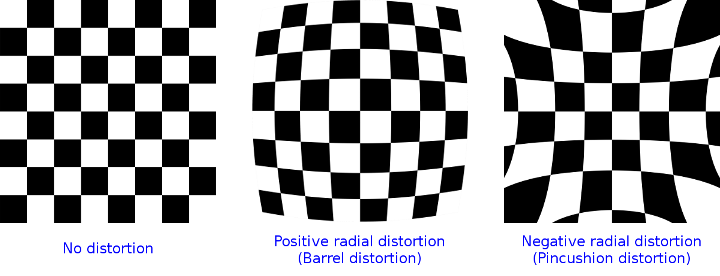
\includegraphics[width=\textwidth]{media/distortion_examples}\\
\caption{\textbf{Radiale Verzerrung Beispiel \autocite{OpencvCamera2016}}
}
\label{Fig:radialdistortion}
\end{figure}

Um nun den tatsächlichen Bildpunkt zu erhalten, müssen also noch diese Parameter berücksichtigt werden. Damit ergibt sich:
$sk = A [R | t] * P 
$
wobei $A = \begin{bmatrix} f_x & \gamma & c_x \\
                             0 &  f_y   & c_y \\
                             0 &  0     &  1\end{bmatrix}$ und $s$ ein Skalierungsfaktor ist, abhängig von der Auflösung. $\gamma$ gibt an in welchem Winkel die Image Plane zum Kamera Koordinatensystem rotiert ist. Zuletzt wird nun der eigentliche Bildpunkt, bzw. Pixel errechnet, indem $m=(x/z, y/z)=(u,v)$.



\subsection{Programmierung von Computer Vision}
\label{sec:opencv}
Da es viele Basisprobleme und Anwendungen in der Computer Vision gibt wurde eine open source Library implementiert. Die geläufigste ist die Open Source Computer Vision Library, kurz OpenCV, sie wurde unter BSD Lizenz veröffentlicht, sodass sie nahezu ohne Einschränkungen genutzt werden kann. Die Bibliothek ist größtenteils in C\# und C++  geschrieben und wurd anfänglich von Intel entwickelt wurde. \textbf{\autocite[512--]{Medioni:2004:ETC:993884} }Einige Gründe hierfür waren der Wunsch der Forschungsgemeinschaft zu ermöglichen neue Anwendungen implementieren zu können ohne sich um die grundlegende Implementierung kümmern zu müssen. So bietet OpenCV auch Möglichkeiten um eine Kamera mit einfachen Mitteln kalibrieren zu können. Auf das Vorgehen dabei wird in \prettyref{sec:camera} eingegangen.
Die Bibliothek ist auf allen Gängigen Betriebssystemen verfügbar, so gibt eine Windows, Linux/Mac Version. Zudem gibt es für mobile Applikationen noch eine Unterstützung von Android.

Für OpenCV sind Interfaces zu anderen Sprachen implementiert worden. So ist es möglich OpenCV in Java und Python zu nutzen. \autocite{OpenCV2016} Insgesamt werden rund 2500 optimierte Algorithmen angeboten, hierzu zählen Algorithmen im Bereich Maschine Learning, 3D Objekt Erkennung, Gesichtserkennung und vielem mehr. Zudem befinden sich Interfaces zu Nvidias CUDA, eine Bibliothek zur Parallelen Berechnung \autocite{cuda2017}, und zu OpenCL aktuell in der aktiven Entwicklung.
\todo{opencv Benutzung erklären}


\section{Aufbau der Testumgebung}
\label{sec:setup}
Im folgenden ein kurzer Abriss über die Umgebung, die als Basis diente um die Entwicklung für diese Arbeit vorzunehmen. 



